\documentclass[aspectratio=169]{beamer}

\usetheme{Boadilla}
\usefonttheme{professionalfonts}
\setbeamertemplate{navigation symbols}{}
\setbeamertemplate{itemize items}[circle]
\setbeamertemplate{enumerate items}[default]
\setbeamertemplate{headline}{}

\usepackage[utf8]{inputenc}
\usepackage[T1]{fontenc}
\usepackage{lmodern}
\usepackage{amsmath}
\usepackage{booktabs}
\usepackage{tabularx}
\usepackage{array}
\usepackage{hyperref}
\usepackage[strings]{underscore}
\usepackage{listings}
\usepackage{tikz}
\usetikzlibrary{arrows.meta,positioning,fit,calc,shapes.geometric}
\usepackage{xcolor}

\definecolor{courseblue}{HTML}{12355B}
\definecolor{coursegold}{HTML}{C98A2E}
\definecolor{courseice}{HTML}{EEF3F8}
\definecolor{coursegreen}{HTML}{2F6B4F}
\definecolor{coursegray}{HTML}{4B5563}
\definecolor{codebg}{HTML}{F7F9FC}
\definecolor{codecomment}{HTML}{5E6C84}
\definecolor{codestring}{HTML}{0B6E4F}

\setbeamercolor{palette primary}{bg=courseblue,fg=white}
\setbeamercolor{palette secondary}{bg=coursegold,fg=white}
\setbeamercolor{palette tertiary}{bg=courseblue,fg=white}
\setbeamercolor{palette quaternary}{bg=coursegold,fg=white}
\setbeamercolor{structure}{fg=courseblue}
\setbeamercolor{frametitle}{bg=courseice,fg=courseblue}
\setbeamercolor{title}{fg=courseblue}
\setbeamercolor{block title}{bg=courseblue,fg=white}
\setbeamercolor{block body}{bg=courseice,fg=black}
\setbeamercolor{normal text}{fg=black,bg=white}
\setbeamercolor{alerted text}{fg=coursegold}

\setbeamerfont{footline}{size=\scriptsize}

\setbeamertemplate{footline}{
  \leavevmode
  \hbox{
    \begin{beamercolorbox}[wd=.33\paperwidth,ht=2.8ex,dp=1.2ex,leftskip=0.8em]{palette primary}%
      University of Trieste
    \end{beamercolorbox}%
    \begin{beamercolorbox}[wd=.49\paperwidth,ht=2.8ex,dp=1.2ex,center]{palette tertiary}%
      \coursename{} \textbar{} \coursecode
    \end{beamercolorbox}%
    \begin{beamercolorbox}[wd=.18\paperwidth,ht=2.8ex,dp=1.2ex,rightskip=0.8em plus1fil]{palette secondary}%
      \insertframenumber{} / \inserttotalframenumber
    \end{beamercolorbox}%
  }
}

\hypersetup{
  colorlinks=true,
  linkcolor=courseblue,
  urlcolor=coursegreen
}

\lstdefinestyle{coursepython}{
  language=Python,
  basicstyle=\ttfamily\footnotesize,
  keywordstyle=\color{courseblue}\bfseries,
  commentstyle=\color{codecomment}\itshape,
  stringstyle=\color{codestring},
  showstringspaces=false,
  columns=fullflexible,
  keepspaces=true,
  frame=single,
  framerule=0.6pt,
  rulecolor=\color{courseblue},
  backgroundcolor=\color{codebg},
  xleftmargin=0.4em,
  xrightmargin=0.4em,
  aboveskip=0.4em,
  belowskip=0.2em
}

\newcommand{\coursename}{Data-driven Systems Engineering}
\newcommand{\coursecode}{440MI / 305SM}
\newcommand{\coursefooter}{}

\newcommand{\learninggoals}[1]{
  \begin{block}{Learning goals}
  #1
  \end{block}
}

\newcommand{\repoactivity}[1]{
  \begin{block}{Repo activity}
  #1
  \end{block}
}

\newcommand{\readinglist}[1]{
  \begin{block}{Papers and materials}
  {\footnotesize #1}
  \end{block}
}

\newcommand{\coursecontextframe}[5]{
  \begin{frame}{Course Map and Running Cases}
  \centering
  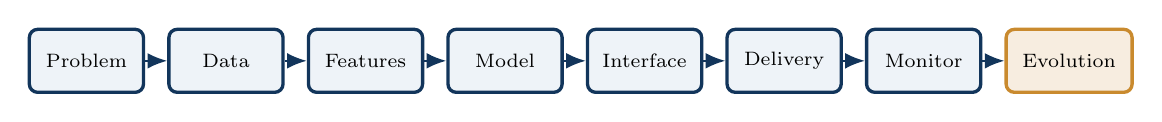
\begin{tikzpicture}[node distance=0.28cm]
  \node[flowbox, minimum width=1.45cm, minimum height=0.8cm] (problem) {\scriptsize Problem};
  \node[flowbox, minimum width=1.45cm, minimum height=0.8cm, right=of problem] (data) {\scriptsize Data};
  \node[flowbox, minimum width=1.45cm, minimum height=0.8cm, right=of data] (features) {\scriptsize Features};
  \node[flowbox, minimum width=1.45cm, minimum height=0.8cm, right=of features] (model) {\scriptsize Model};
  \node[flowbox, minimum width=1.45cm, minimum height=0.8cm, right=of model] (interface) {\scriptsize Interface};
  \node[flowbox, minimum width=1.45cm, minimum height=0.8cm, right=of interface] (delivery) {\scriptsize Delivery};
  \node[flowbox, minimum width=1.45cm, minimum height=0.8cm, right=of delivery] (monitor) {\scriptsize Monitor};
  \node[accentbox, minimum width=1.6cm, minimum height=0.8cm, right=of monitor] (evolution) {\scriptsize Evolution};
  \foreach \a/\b in {problem/data,data/features,features/model,model/interface,interface/delivery,delivery/monitor,monitor/evolution} {
    \draw[arrow] (\a) -- (\b);
  }
  \end{tikzpicture}

  \vspace{0.5em}
  \begin{block}{Today in the course}
  \textbf{Focus:} #1

  \textbf{Bridge:} #2
  \end{block}

  \begin{columns}[T]
  \column{0.48\textwidth}
  \begin{block}{Fraud case}
  {\footnotesize #3}
  \end{block}
  \column{0.48\textwidth}
  \begin{block}{Pasteurization case}
  {\footnotesize #4}
  \end{block}
  \end{columns}

  \vspace{0.3em}
  {\footnotesize \textbf{Course thread:} #5}
  \coursefooter
  \end{frame}
}

\newcommand{\classclosingframe}[4]{
  \begin{frame}{From This Class to the Next}
  \begin{block}{What stays with us}
  #1
  \end{block}

  \begin{columns}[T]
  \column{0.48\textwidth}
  \begin{block}{Project use}
  {\footnotesize #2}
  \end{block}
  \column{0.48\textwidth}
  \begin{block}{Next connection}
  {\footnotesize #3}
  \end{block}
  \end{columns}

  \vspace{0.3em}
  {\footnotesize \textbf{Course thread:} #4}
  \coursefooter
  \end{frame}
}

\tikzset{
  flowbox/.style={
    rounded corners=3pt,
    draw=courseblue,
    fill=courseice,
    very thick,
    minimum width=2.2cm,
    minimum height=0.9cm,
    align=center,
    font=\small
  },
  accentbox/.style={
    rounded corners=3pt,
    draw=coursegold,
    fill=coursegold!15,
    very thick,
    minimum width=2.2cm,
    minimum height=0.9cm,
    align=center,
    font=\small
  },
  arrow/.style={
    -{Latex[length=2.5mm,width=2mm]},
    thick,
    draw=courseblue
  }
}


\title{Class 18: Online Learning and Concept Drift}
\author{\coursename}
\date{}

\begin{document}

\frame{\titlepage \coursefooter}

\begin{frame}{Agenda}
\begin{itemize}
\item Why a validated model can still go stale.
\item Offline versus online (incremental) learning.
\item River: learning one observation at a time.
\item Concept drift: what it is, and how ADWIN detects it.
\item Monitoring a streaming model with River and Evidently together.
\end{itemize}
\coursefooter
\end{frame}

\begin{frame}{Learning goals}
\learninggoals{
\begin{itemize}
\item Explain why some systems need incremental learning instead of periodic retraining.
\item Use River's `predict\_one` / `learn\_one` pattern to reason about streaming models.
\item Define concept drift and distinguish it from ordinary noise.
\item Connect a drift detector such as ADWIN to a concrete monitoring and reset action.
\end{itemize}
}
\coursefooter
\end{frame}

\coursecontextframe
{Learning continuously from streams, and detecting when the data itself has changed.}
{Class 17 evaluated a fixed, trained model. This class asks what happens once that model has to keep working as new data keeps arriving.}
{The fraud case can use periodic batch retraining, but spending patterns and fraud tactics still drift over time between retraining cycles.}
{The pasteurization case is a natural streaming problem: sensors arrive continuously, and process or calibration changes must be detected as they happen.}
{The course thread now shifts from a single validated snapshot to a model that must keep validating itself over time.}

\begin{frame}{Offline versus online learning}
\begin{columns}[T]
\column{0.48\textwidth}
\textbf{Offline}
\begin{itemize}
\item Train on a fixed dataset
\item Easier benchmarking
\item Periodic retraining
\end{itemize}
\column{0.48\textwidth}
\textbf{Online}
\begin{itemize}
\item Update one sample at a time
\item Works directly on streams
\item Responds faster to change
\end{itemize}
\end{columns}
\coursefooter
\end{frame}

\begin{frame}{Why adaptation becomes necessary}
\begin{itemize}
\item User behavior changes.
\item Sensors drift or get recalibrated.
\item Business policies or regulations shift.
\item New classes of errors appear only after deployment.
\end{itemize}
\begin{block}{Key point}
Model adaptation is not a sign that the first model failed. It is a recognition that the environment keeps evolving.
\end{block}
\coursefooter
\end{frame}

\begin{frame}[fragile]{River example: incremental regression}
\begin{lstlisting}[style=coursepython]
model = preprocessing.StandardScaler() | linear_model.LinearRegression(
    optimizer=optim.SGD(0.01)
)
mae = metrics.MAE()

y_pred = model.predict_one(x)
model.learn_one(x, y)
mae.update(y, y_pred)
\end{lstlisting}
\begin{itemize}
\item From `notebooks/Class8_Model_Incremental_learning.ipynb`: the model predicts, then learns, one observation at a time.
\item There is no fixed training set; the model's parameters update continuously as data arrives from the Open-Meteo API.
\end{itemize}
\coursefooter
\end{frame}

\begin{frame}{What is concept drift?}
\begin{itemize}
\item Concept drift is a change in the statistical relationship between inputs and target over time, not just noisy individual readings.
\item Sudden drift: an abrupt regime change, such as a sensor recalibration or a new fraud pattern appearing overnight.
\item Gradual drift: a slow shift, such as seasonal changes in spending or a wearing physical sensor.
\item A model trained before the drift can keep looking confident while its predictions quietly become wrong.
\end{itemize}
\coursefooter
\end{frame}

\begin{frame}{The streaming learning loop}
\centering
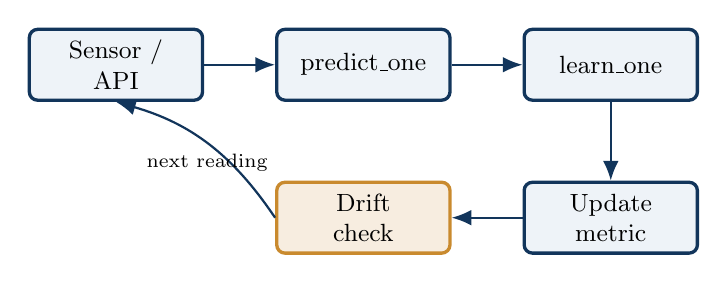
\begin{tikzpicture}[node distance=1cm and 0.9cm]
\node[flowbox] (source) {Sensor /\\API};
\node[flowbox, right=of source] (predict) {predict\_one};
\node[flowbox, right=of predict] (learn) {learn\_one};
\node[flowbox, below=of learn] (metric) {Update\\metric};
\node[accentbox, left=of metric] (drift) {Drift\\check};
\draw[arrow] (source) -- (predict);
\draw[arrow] (predict) -- (learn);
\draw[arrow] (learn) -- (metric);
\draw[arrow] (metric) -- (drift);
\draw[arrow, bend right=20] (drift.west) to node[below, font=\scriptsize] {next reading} (source.south);
\end{tikzpicture}
\coursefooter
\end{frame}

\begin{frame}[fragile]{River example: ADWIN drift detection}
\begin{lstlisting}[style=coursepython]
adwin = drift.ADWIN(delta=0.002)
...
error = abs(y - (y_pred or 0))
adwin.update(error)

if adwin.drift_detected:
    print("Resetting model due to detected drift...")
    model = preprocessing.StandardScaler() | linear_model.LinearRegression(
        optimizer=optim.SGD(0.01)
    )
    adwin = drift.ADWIN(delta=0.002)
\end{lstlisting}
\begin{itemize}
\item From `notebooks/Class8_Model_Incremental_learning.ipynb`: ADWIN watches the prediction error stream and flags a statistically significant change.
\item Detecting drift is only half the job; the notebook resets both the model and the detector once drift fires.
\end{itemize}
\coursefooter
\end{frame}

\begin{frame}{Why ADWIN and similar detectors matter}
\begin{itemize}
\item ADWIN keeps an adaptive window of recent errors and compares its sub-windows for a statistically significant change.
\item It grows the window while things look stable and shrinks it the moment the error distribution shifts.
\item This gives a principled trigger for retraining or resetting, instead of a fixed, arbitrary retraining schedule.
\end{itemize}
\coursefooter
\end{frame}

\begin{frame}[fragile]{From notebook to dashboard: the same pattern, deployed}
\begin{lstlisting}[style=coursepython]
y_pred = model.predict_one(x)
model.learn_one(x, y)
adwin.update(abs(temp - (y_pred or 0)))
drift_flag = adwin.drift_detected
\end{lstlisting}
\begin{itemize}
\item From `streamlit/pages/App_Stream.py`: the exact same River and ADWIN pattern from the notebook, now driving a live dashboard.
\item Detected drift points are plotted directly against the mean absolute error curve, so an operator sees drift, not just a number.
\end{itemize}
\coursefooter
\end{frame}

\begin{frame}{Monitoring beyond a single detector}
\begin{itemize}
\item `notebooks/Class8_Model_Incremental_learning.ipynb` also integrates Evidently's `DataDriftPreset` and `DataQualityPreset` reports alongside River.
\item A single statistical test (ADWIN on the error) is a fast, targeted signal; a full drift report checks many columns and quality dimensions at once.
\item Combining a lightweight online detector with periodic, richer reports is a realistic production pattern, not an either-or choice.
\end{itemize}
\coursefooter
\end{frame}

\begin{frame}{Batch retraining versus online learning}
\begin{tabularx}{\textwidth}{>{\bfseries}l X}
Latency to adapt & Online reacts immediately; batch waits for the next retraining cycle. \\
Auditability & Batch snapshots are easy to freeze and review; online state changes continuously. \\
Risk of instability & Online models can overreact to noise if the detector is too sensitive. \\
Infrastructure cost & Online avoids large periodic retraining jobs but needs always-on serving. \\
\end{tabularx}
\coursefooter
\end{frame}

\begin{frame}{Where drift shows up in the two running cases}
\begin{itemize}
\item Fraud: seasonal spending shifts, new merchant categories, or fraud rings adopting a new pattern.
\item Pasteurization: sensor recalibration, raw-material changes, or wear in the heating and cooling equipment.
\item In both cases, drift detection turns ``the model got worse'' from a mystery into a specific, timestamped event.
\end{itemize}
\coursefooter
\end{frame}

\begin{frame}{Repository connections}
\repoactivity{
\begin{itemize}
\item `notebooks/Class8_Model_Incremental_learning.ipynb` is the primary anchor: River regression, ADWIN, and Evidently reports.
\item `streamlit/pages/App_Stream.py` deploys the same River and ADWIN pattern as a live dashboard.
\end{itemize}
}
\coursefooter
\end{frame}

\begin{frame}{Discussion prompt}
\begin{block}{Question}
ADWIN just fired on the pasteurization temperature stream. Is that a sensor fault, a process change, or a false alarm, and how would you tell the difference?
\end{block}
\begin{itemize}
\item This connects drift detection back to the state-machine and signal reasoning from Class 13.
\end{itemize}
\coursefooter
\end{frame}

\begin{frame}{Papers and materials}
\readinglist{
\href{https://riverml.xyz/latest/}{River documentation};\
\href{https://riverml.xyz/latest/api/drift/ADWIN/}{River ADWIN documentation};\
\href{https://riverml.xyz/latest/api/metrics/}{River metrics API};\
\href{https://arxiv.org/abs/2007.06299}{Gama et al., A survey on concept drift adaptation};\
\href{https://evidentlyai.com/blog/data-drift-detection-large-datasets}{Evidently on data drift detection}.
}
\coursefooter
\end{frame}

\classclosingframe
{\begin{itemize}
\item Online learning updates a model one observation at a time, trading offline benchmarking convenience for responsiveness.
\item Concept drift is a real, detectable statistical event, not a vague excuse for degraded performance.
\item ADWIN-style detectors give a principled trigger for retraining or resetting a model.
\end{itemize}}
{Project teams should decide, for their own case, whether periodic retraining is enough or whether an online or drift-aware component is warranted.}
{Class 19 is a hands-on lab: generating, serving, and streaming the pasteurization sensors that this class's drift ideas were grounded in.}
{Detecting drift only matters if there is a running streaming system to detect it in, which is exactly what the next class builds.}

\end{document}
